\begin{table}[htbp]
\centering
\caption{Propensity score overlap diagnostics}
\label{tab:overlap_diagnostics}
\small
\begin{minipage}[t]{0.41\textwidth}
\vspace{0pt}
\centering
\begin{threeparttable}
\begin{tabular}{lr}
\toprule
Metric & Value \\
\midrule
Observations & 23,971 \\
Treated observations & 12,720 \\
Control observations & 11,251 \\
Treated share & 0.531 \\
PS minimum & 0.060 \\
PS 1st percentile & 0.197 \\
PS 99th percentile & 0.821 \\
PS maximum & 0.943 \\
Overlap lower bound & 0.343 \\
Overlap upper bound & 0.713 \\
Share with \(e(X)\le 0.03\) & 0.000 \\
Share with \(e(X)\ge 0.97\) & 0.000 \\
\bottomrule
\end{tabular}
\end{threeparttable}
\end{minipage}
\hfill
\begin{minipage}[t]{0.55\textwidth}
\vspace{0pt}
\centering
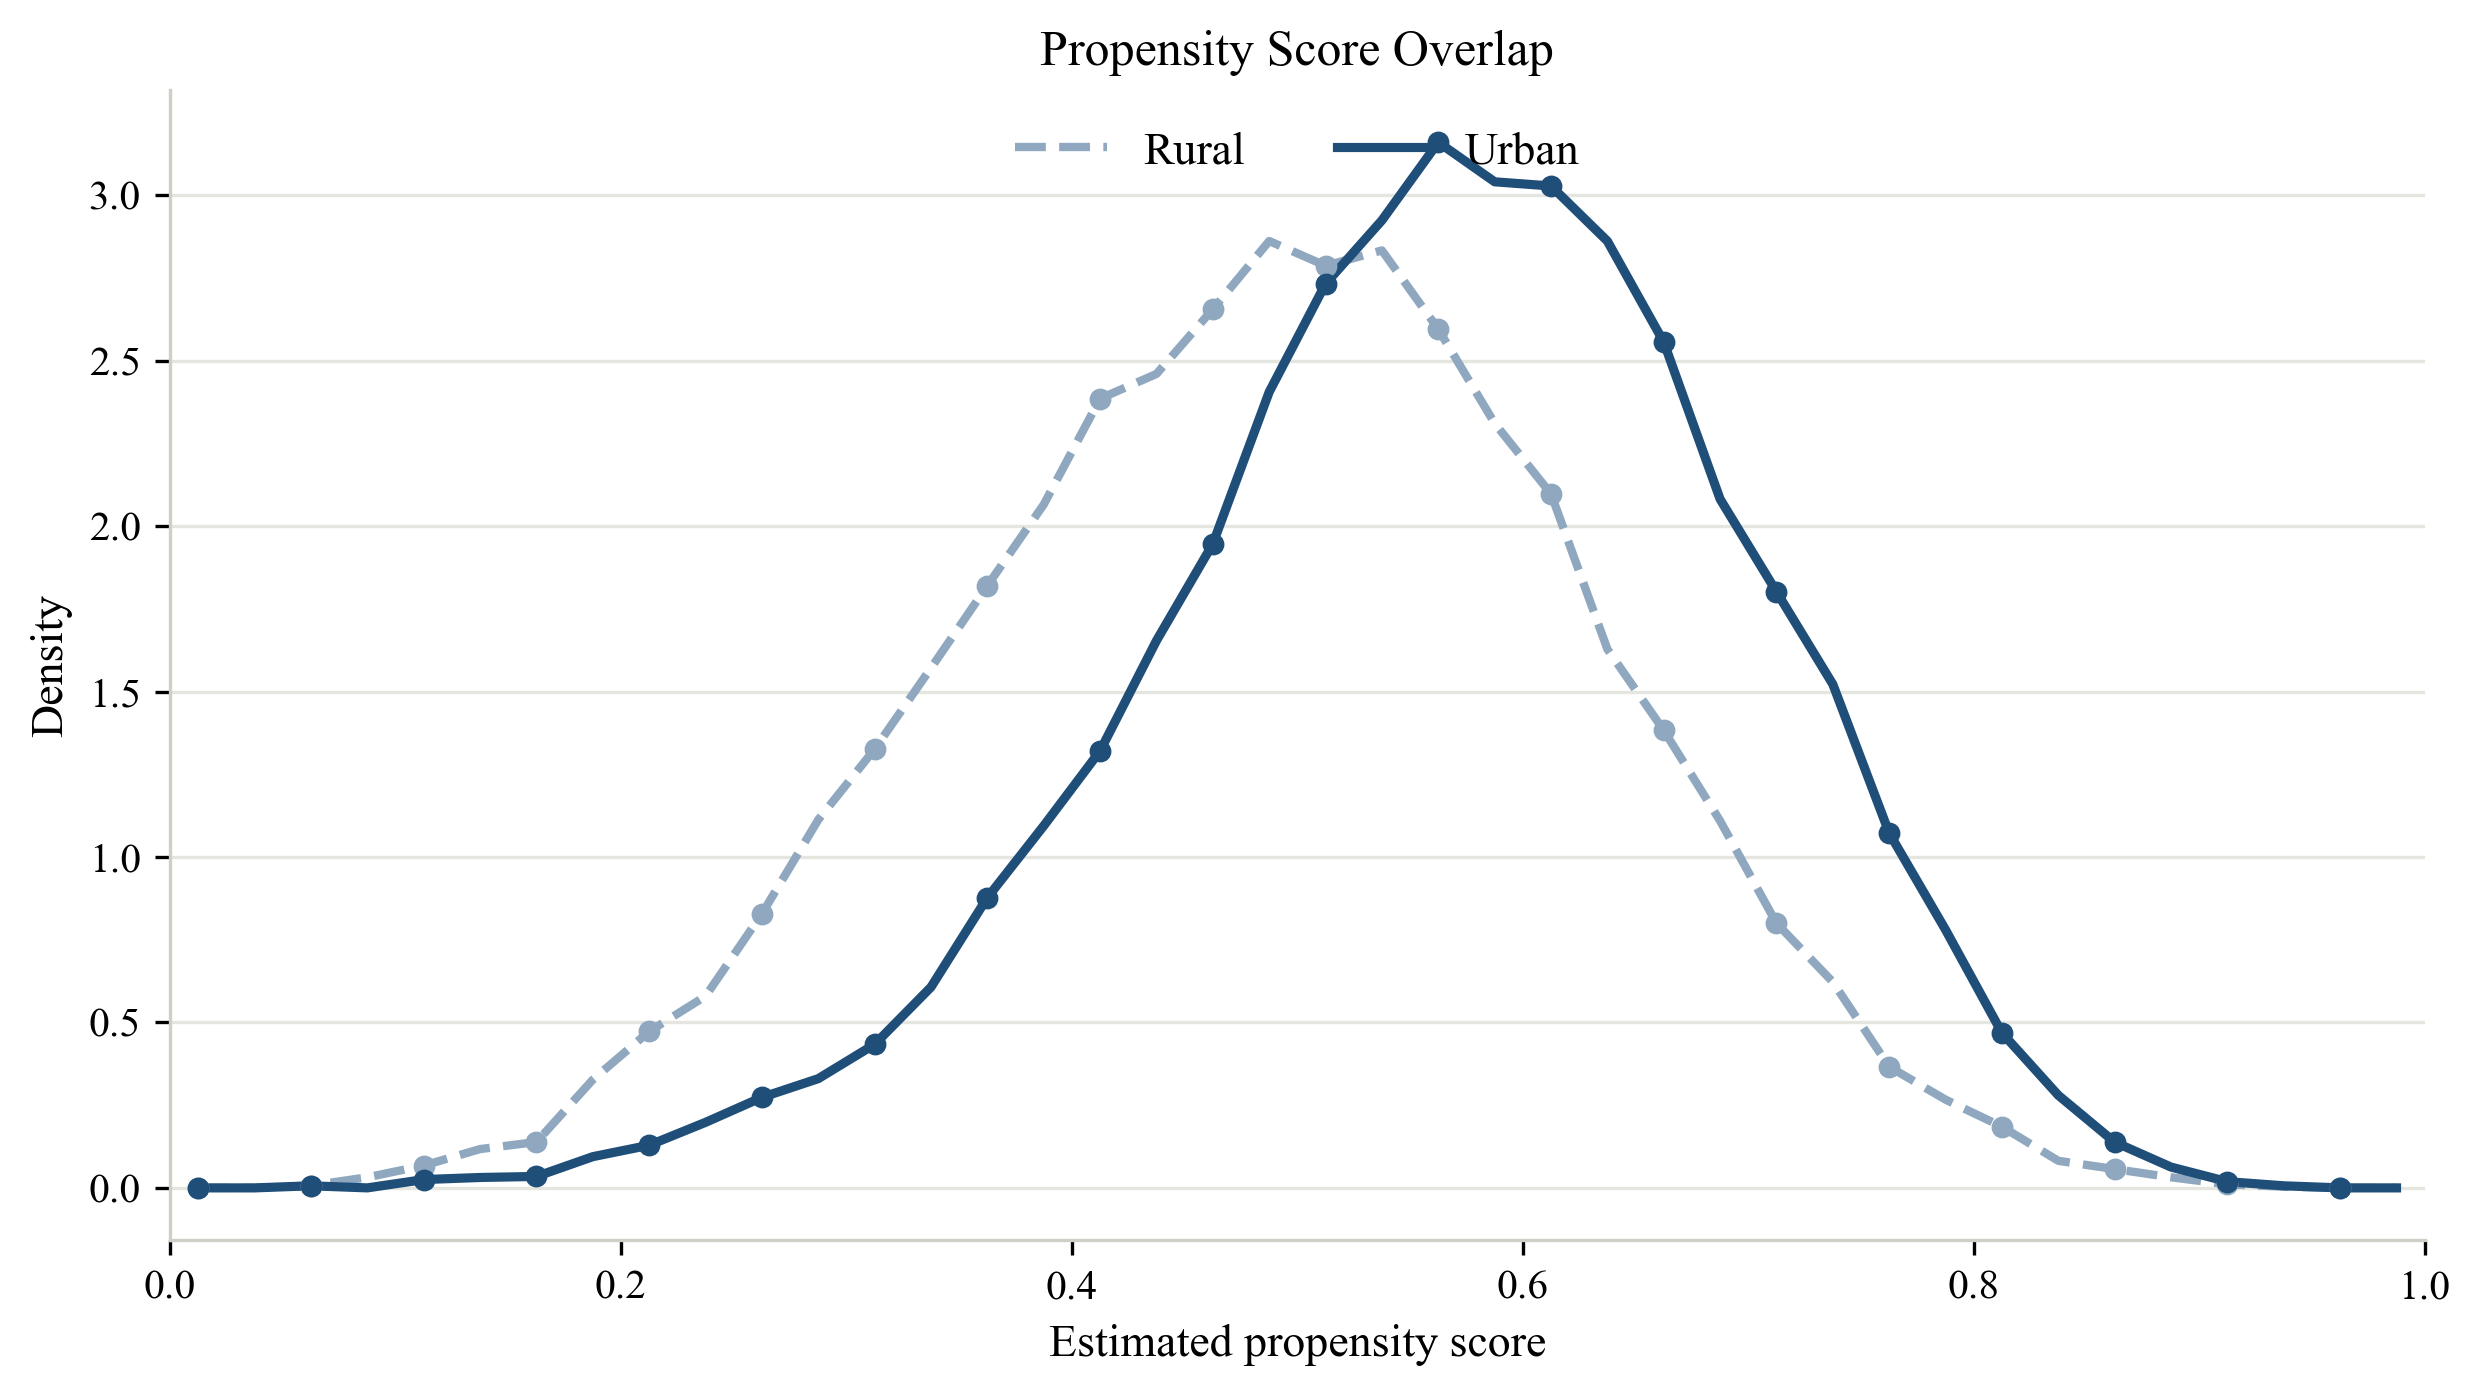
\includegraphics[width=\textwidth]{latex/propensity_overlap_plot.png}
\end{minipage}

\begin{minipage}{0.97\textwidth}
\vspace{0.4em}
\footnotesize
Notes: The left panel reports summary diagnostics for the estimated propensity score in the main analysis sample. The right panel shows the propensity score distributions for urban and rural households.
\end{minipage}
\end{table}
